\documentclass[12pt]{article}
\setlength\parindent{0pt}
\usepackage{fullpage}
\usepackage{graphicx}
\usepackage{amsmath}
\setlength{\parskip}{4mm}
\def\LL{\left\langle}   % left angle bracket
\def\RR{\right\rangle}  % right angle bracket
\def\LP{\left(}         % left parenthesis
\def\RP{\right)}        % right parenthesis
\def\LB{\left\{}        % left curly bracket
\def\RB{\right\}}       % right curly bracket
\def\PAR#1#2{ {{\partial #1}\over{\partial #2}} }
\def\PARTWO#1#2{ {{\partial^2 #1}\over{\partial #2}^2} }
\def\PARTWOMIX#1#2#3{ {{\partial^2 #1}\over{\partial #2 \partial #3}} }
\newcommand{\BE}{\begin{displaymath}}
	\newcommand{\EE}{\end{displaymath}}
\newcommand{\BNE}{\begin{equation}}
	\newcommand{\ENE}{\end{equation}}
\newcommand{\BEA}{\begin{eqnarray}}
	\newcommand{\EEA}{\nonumber\end{eqnarray}}
\newcommand{\EL}{\nonumber\\}
\newcommand{\la}[1]{\label{#1}}
\newcommand{\ie}{{\em i.e.\ }}
\newcommand{\eg}{{\em e.\,g.\ }}
\newcommand{\cf}{cf.\ }
\newcommand{\etc}{etc.\ }
\newcommand{\Tr}{{\rm tr}}
\newcommand{\etal}{{\it et al.}}
\newcommand{\OL}[1]{\overline{#1}\ } % overline
\newcommand{\OLL}[1]{\overline{\overline{#1}}\ } % double overline
\newcommand{\OON}{\frac{1}{N}} % "one over N"
\newcommand{\OOX}[1]{\frac{1}{#1}} % "one over X"



\begin{document}
	\Large
	\centerline{\sc{Homework 6}}
	\normalsize
	\centerline{\sc{Due Wednesday, 30 March, in recitation}}
	
	\begin{enumerate}
		
		\item{We saw in class that in a pendulum the string does no work. We also saw that the normal force does no work on an object sliding down a ramp.}
		\begin{enumerate}
			\item{Explain why the tension in the string of a pendulum does no work.}
			\item{Explain why the normal force does no work on an object sliding down a ramp.}
			\item{Give an example of a situation where tension {\it does} do work on an object.}
			\item{Give an example of a situation where friction does positive work on something.}
		\end{enumerate}

\item On a cold winter day, you might rub your hands together to warm them up. The kinetic friction as you rub your hands together does negative work on your hands.
The law of conservation of energy says that energy is never lost, only converted from one form to another; in this case,
this energy is dissipated as heat. 
\begin{enumerate}
\item Estimate the power (in joules per second) produced by this process. You will need to make quite a few estimates here involving the
parameters of rubbing your hands together; tell me what they are in your solution. (There are no right and wrong answers here; we are interested in your thought process.)
\item It requires about four joules of added heat to raise the temperature of one gram of tissue by one degree Celsius (1.8 degrees Fahrenheit). 
Is rubbing your hands together an effective way to keep your hands warm?
What about your whole body? Again, tell me what approximations and assumptions you make here. 
\end{enumerate}

 \item{A lazy penguin slides down a snow-covered slope on its chest. Suppose that the diagonal length of the slope is 12 m, and it is inclined at an angle of $10^o$ above the horizontal. If the penguin is traveling at 4 m/s when it 
	reaches the bottom of the slope, what is the coefficient of friction between the penguin and the slope? Do this problem twice: once with Newton's second law and kinematics, and once with energy methods. Write a few sentences comparing the 
	approaches.}

\item{Imagine that our same lazy penguin slides down another ice-covered slope. The coefficient of kinetic friction is $\mu_k$.
	This slope is inclined at an angle $\theta$ above the horizontal and has a total length $L$. At the bottom of the slope, she keeps going, sliding past the end of the slope along the flat ground until friction brings her to a stop.
	
	How far will she travel past the end of the slope before friction brings her to rest?}


\item{A person uses a block-and-tackle system as shown below (from Wikimedia Commons) to lift a heavy load.
	
	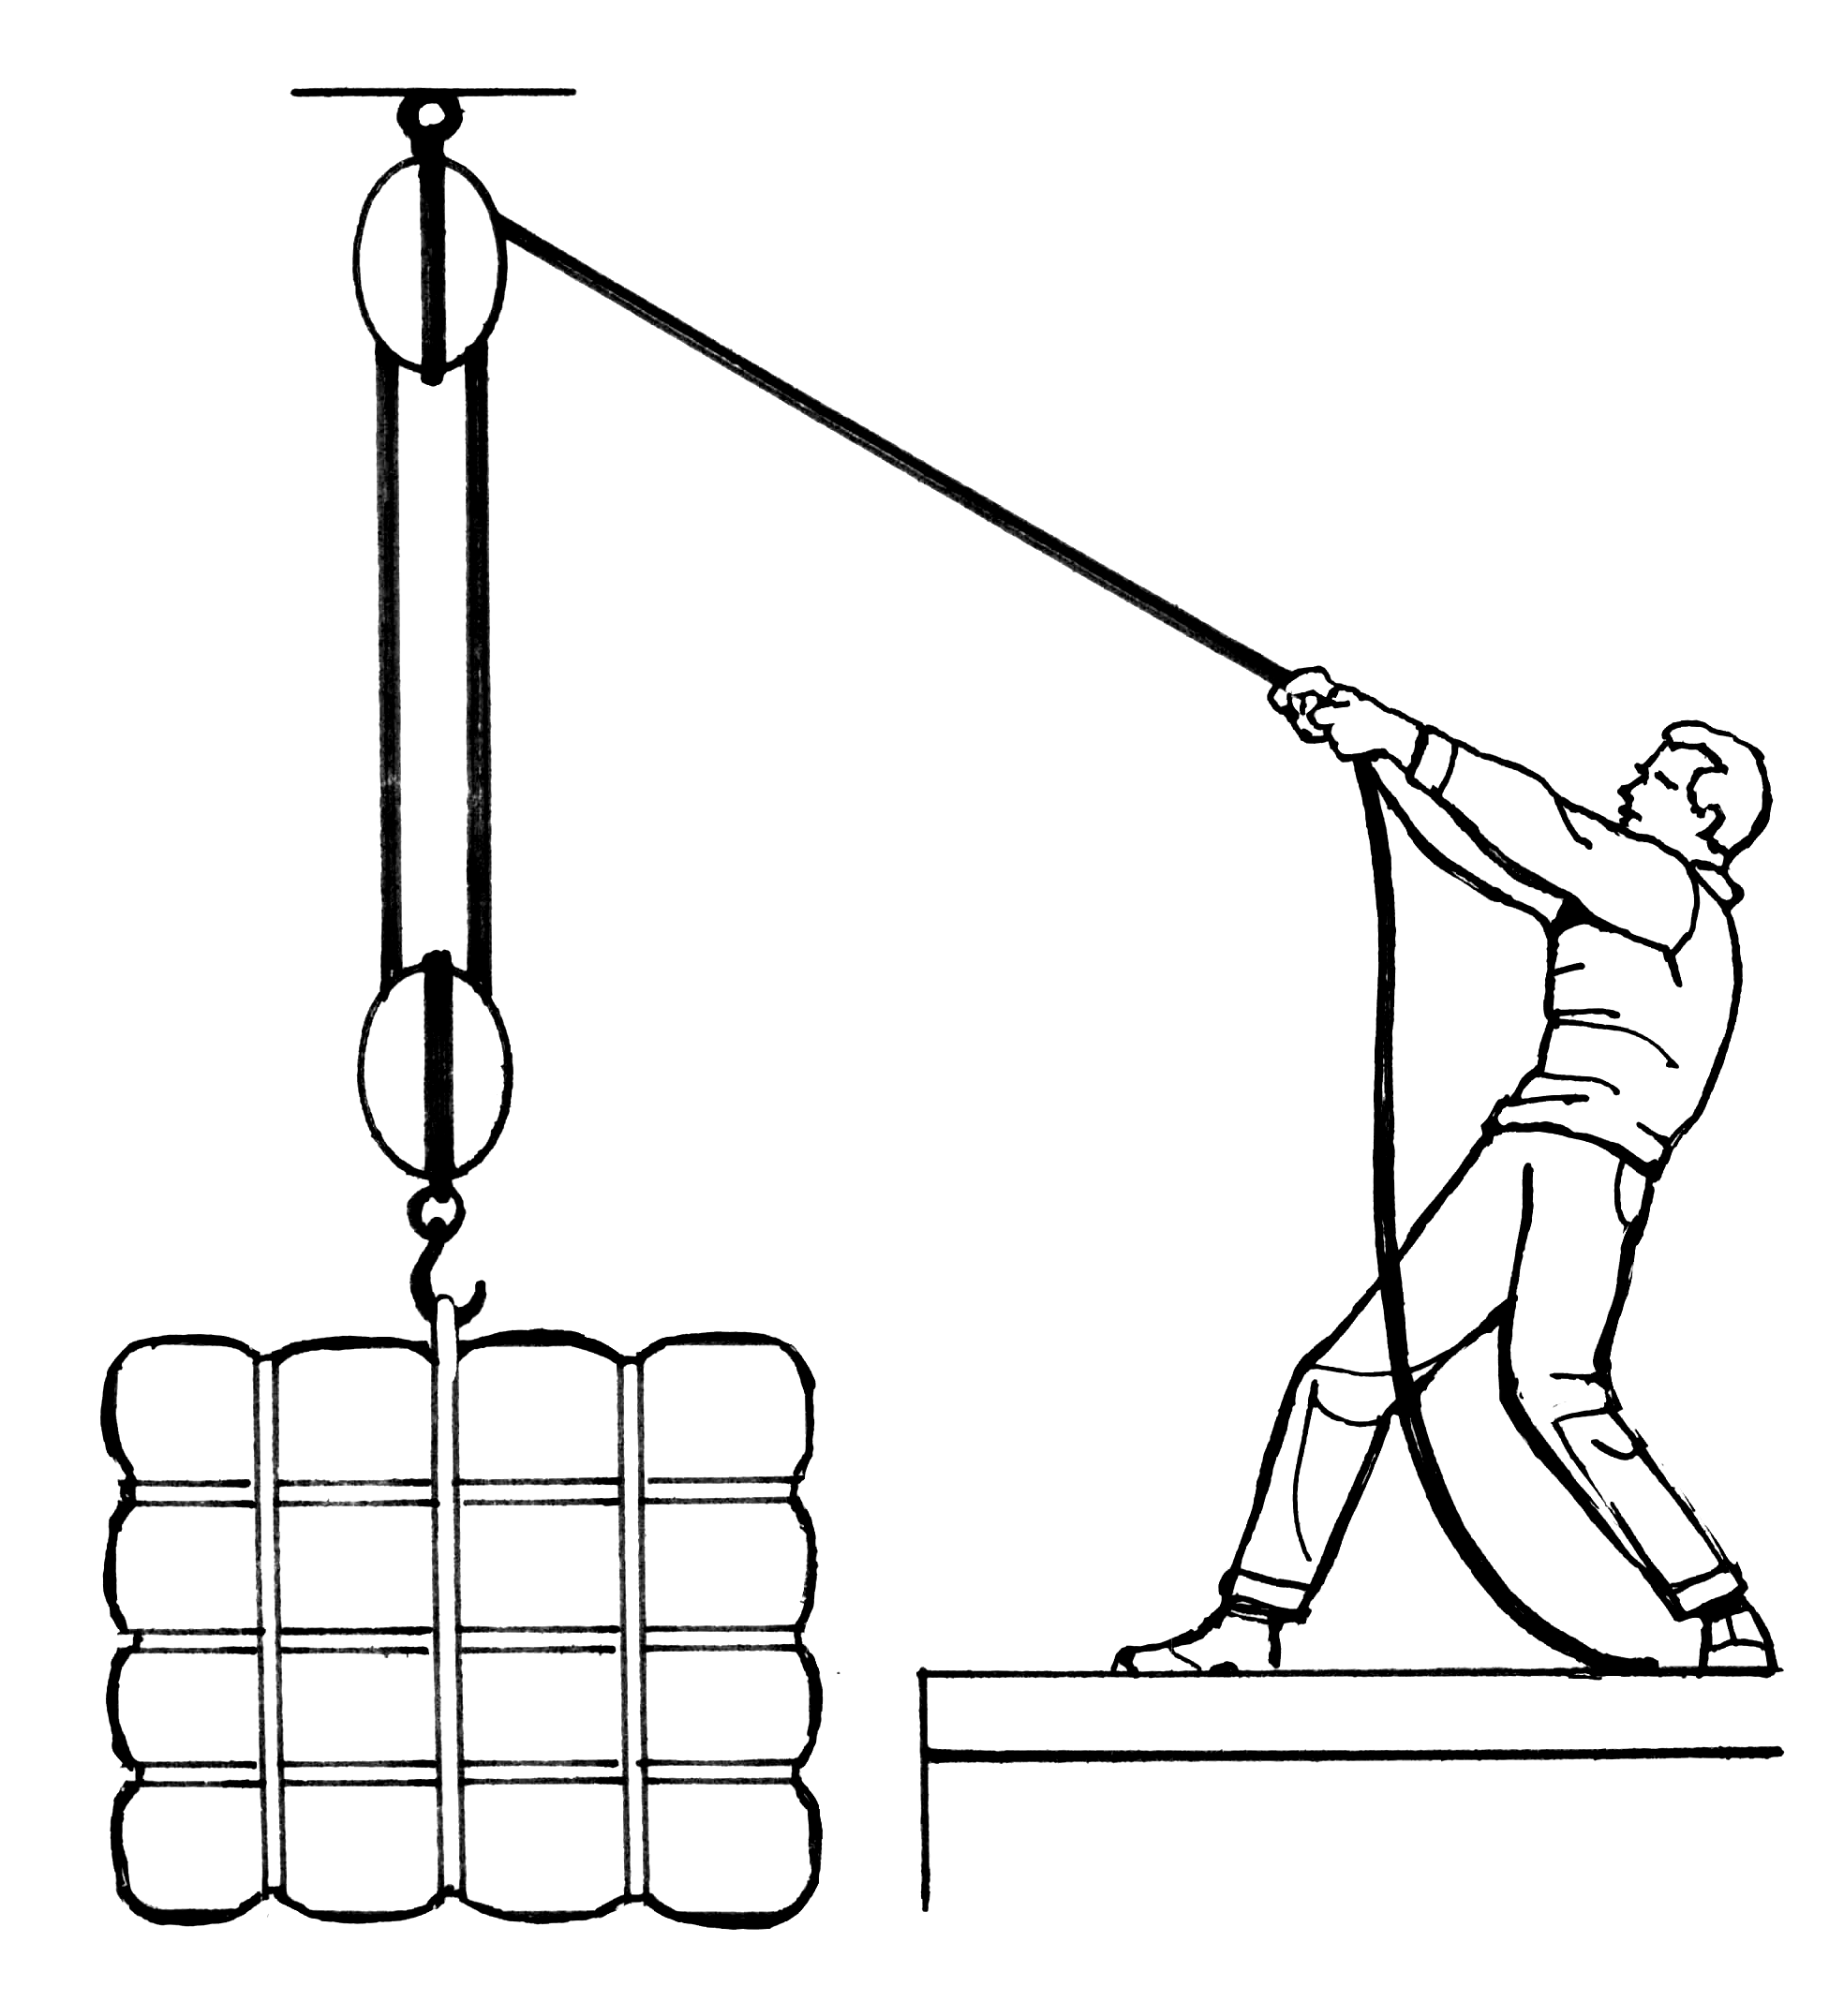
\includegraphics[width=0.3\textwidth]{blockandtackle.png}
	
	Suppose the load has a weight of 1250 N. 
	
	\begin{enumerate}
		\item{Suppose our person lifts this load two meters slowly (at constant velocity). What force must he exert on the rope to do so?} 
		\item{It seems like he's getting something for nothing -- that he's able to lift a larger weight with a smaller force. But is he? Calculate the work done by the rope on the load, and calculate the work he does on the rope.}
		\item{If he lifts this load 2m and then holds it there, clearly its change in kinetic energy is zero: it started at rest and ended at rest. However, the rope did positive work on the load; the work-energy theorem thus says that its kinetic energy should
			increase unless some other force did an equal amount of negative work on it. What force was this?}
		\item{Explain why, using the definition of work $W = \int \vec F \cdot d\vec s$, that force does negative work.}
	\end{enumerate}
}

\item Electric cars like the Tesla Model 3 or Chevrolet Bolt have battery capacities measured in ``kilowatt-hours''. The long-range model of the Model 3 has a battery rated at 75 kilowatt-hours. 
\begin{enumerate}
	\item Using dimensional analysis, what sort of quantity (time, force, power, energy, distance, etc.) might be measured in kilowatt-hours? Convert one kilowatt-hour into more familiar units.
	\item The US Environmental Protection Agency estimates that a Model 3 can drive 523 km (325 miles) on a charge of its battery. If this is the case, estimate the size of the drag force applied to the car by the air it is driving through. How does this force
	compare with the weight of a person?
	\item If this car drives at 110 km/hr for a trip like this, estimate the power delivered to the wheels by the motor to sustain
	this speed. (Remember that power is the rate of doing work, and is equal to $\vec F \cdot \vec v$.)
\end{enumerate}




\end{enumerate}

\end{document}


